% vim: ts=8 sts=8 sw=4 et tw=75
\chapter{算法实验}
\label{chap:experiments_with_algorithms}
\marginpar{153}

一般而言, 理解事物如何工作的最好方式就是自己动手做一些小实验, 算法学习
就是一个典型的例子: 编写实际代码有助于弄清楚那些容易被伪码掩盖的问题.
不仅如此, 最终得到的程序是可运行的, 通过观察运行结果, 就可以知道算法的
的正确性, 而这是伪码所无法办到的.

Awk 很适合做这种测试工作. 如果某个程序使用 awk 编写, 那我们就可以把精力
集中在算法上, 而不是语言本身. 如果某个算法最终要应用到某个大型程序中,
那么先让算法能够单独地运行起来可能会更有效率. 当需要为某个算法进行调试,
测试与性能评价时, 通常需要构造一些脚手架程序, 在这一方面, awk 是一款
优秀的脚手架构造工具, 它并不关心算法本身是用什么语言实现的.

这一章讨论算法实验. 前半章描述三种排序算法, 这三种算法常常是算法课首
先要介绍的内容, 我们将使用 awk 程序对这些算法进行测试, 性能度量和
刻画. 后半章展示几种拓扑排序算法, 实现 Unix 的文件更新实用程序
\texttt{make}.

\section{排序}
\label{sec:sorting}

这一小节讨论三种著名并且很有用的算法: 插入排序, 快速排序, 以及堆排序.
插入排序非常简单, 但是只有在元素很少的情况下效率才足够高; 快速排序
是最好的通用排序算法之一; 堆排序可以保证即使在最坏的情况下, 也可以拥有
较高的效率. 我们对每一种算法都进行介绍, 并加以实现, 然后再用测试例程
对它们进行测试, 最后评价性能.

\subsection{插入排序}
\label{subsec:insertion_sort}
\cterm{基本概念}. 插入排序的过程类似于给一堆卡片排序: 每次从卡片堆里
拿出一张, 把它插入到手上拿着的牌的合适位置.
\footnote{原文为 Insertion sort is similar
    to the method of sorting a sequence of cards by picking up the cards
    one at a time and inserting each card into its proper position in the
hand}

\cterm{实现}. 下面的代码使用插入排序对数组 \texttt{A[1]}, ...,%
\marginpar{154}%
\texttt{A[n]} 进行升序排列. 第一个动作把输入数据读取到一个数组中,
\texttt{END} 动作调用函数 \texttt{isort} 对数组进行排序, 最后输出排序
结果:
\begin{awkcode}
    # insertion sort 
        { A[NR] = $0 }
    END { isort(A, NR)
          for (i = 1; i <= NR; i++)
              print A[i]
        }

    # isort - sort A[1..n] by insertion
    function isort(A, n,    i, j, t) {
        for (i = 2; i <= n; i++)
            for (j = i; j > 1 && A[j-1] > A[j]; j--) {
                # swap A[j-1] and A[j]
                t = A[j-1]; A[j-1] = A[j]; A[j] = t
            }
    }
\end{awkcode}
\texttt{isort} 函数内的外层循环在每次迭代开始时, 数组\texttt{A} 的元素
\texttt{1} 至元素 \textit{i}\texttt{-1} 就已经处于有序状态. 内层循环每
次迭代
都把当前处于第 \textit{i} 个位置上的元素向前移动, 跳过所有比它大的元素. 
当外层循环结束时, 所有的 \textit{n} 个元素都处于有序状态.

数值或字符串都可以用这个程序进行排序. 但是当输入数据同时含有数值与字符
串时, 就要小心一点 --- 由于强制类型转换, 比较结果可能会让你感到惊讶.

如果数组 \texttt{A} 含有以下 8 个整数:
\begin{file}
    8 1 6 3 5 2 4 7
\end{file}
那么排序的过程如下所示:
\begin{file}
    8|1 6 3 5 2 4 7
    1 8|6 3 5 2 4 7
    1 6 8|3 5 2 4 7
    1 3 6 8|5 2 4 7
    1 3 5 6 8|2 4 7
    1 2 3 5 6 8|4 7
    1 2 3 4 5 6 8|7
    1 2 3 4 5 6 7 8|
\end{file}
竖线符把数组的已排序部分和未排序部分分开.

\cterm{测试}. 应该如何测试 \texttt{isort}? 我们可以每次输入一点数据,
并查看排序结果, 当然, 这样做并没有错, 可是对于任意规模的程序来说, 
这种方法不能做到详尽的测试. 第二种方案是自动生成大量的随机数集合, 
把这些集合作为 \texttt{isort} 的输入数据. 这的确是一个不错的办法,
但是还可以做得更好: 为了测试程序的薄弱环节, 我们还需要构造一些特殊
的测试用例, 用来测试边界与异常情况.
\marginpar{155} 对排序来说, 典型的边界与异常情况包括:
\begin{pattern}
\indent 序列长度为 0 \par
\indent 序列长度为 1 \par
\indent 序列包含 \textit{n} 个随机数 \par
\indent 序列包含 \textit{n} 个已排序的数 \par
\indent 序列包含 \textit{n} 个逆序排列的数 \par
\indent 序列包含 \textit{n} 个相同的数
\end{pattern}

本章的目标之一是展示如何使用 awk 来帮助测试和评价程序. 为了说明, 我们现在
要对排序例程的测试与运行结果评价过程进行自动化.

主要有两种办法来实现测试与评价过程的自动化, 每一种都有它各自的优点. 第一 
种称为 ``批处理模式'': 编写一个程序来运行事先计划好的测试集, 并运用前面提到
的几种排序算法.\footnote{原文为 write a program to execute a pre-planned
    set of tests, exercising the sort function as suggested
above.}
下面的程序可以生成测试数据并检查测试结果. 除了 \texttt{isort}, 还有其他
几个函数, 它们用来生成不同类型的数组, 以及检查排序后的数组是否是有序的.
\begin{awkcode}
    # batch test of sorting routines

    BEGIN {
        print "    0 elements"
        isort(A, 0); check(A, 0)    
        print "    1 element"
        genid(A, 1); isort(A, 1); check(A, 1)
        
        n = 10
        print "    " n " random integers"
        genrand(A, n); isort(A, n); check(A, n)
        
        print "    " n " sorted integers"
        gensort(A, n); isort(A, n); check(A, n)
        
        print "    " n " reverse-sorted integers"
        genrev(A, n); isort(A, n); check(A, n)
        
        print "    " n " identical integers"
        genid(A, n); isort(A, n); check(A, n)
    }

    function isort(A,n,     i,j,t) {
        for (i = 2; i <= n; i++)
            for (j = i; j > 1 && A[j-1] > A[j]; j--) {
                # swap A[j-1] and A[j]
                t = A[j-1]; A[j-1] = A[j]; A[j] = t
            }
    }

\end{awkcode}
\marginpar{156}
\begin{awkcode}
    # test-generation and sorting routines...

    function check(A,n,   i) {
        for (i = 1; i < n; i++)
            if (A[i] > A[i+1])
                printf("array is not sorted, element %d\n", i)
    }

    function genrand(A,n,  i) { # put n random integers in A
        for (i = 1; i <= n; i++)
            A[i] = int(n*rand())
    }

    function gensort(A,n,  i) { # put n sorted integers in A
        for (i = 1; i <= n; i++)
            A[i] = i
    }

    function genrev(A,n,  i) {  # put n reverse-sorted integers
        for (i = 1; i <= n; i++)  # in A
            A[i] = n+1-i
    }

    function genid(A,n,  i) {   # put n identical integers in A
        for (i = 1; i <= n; i++)
            A[i] = 1
    }
\end{awkcode}

第二种方法相对来说没那么方便, 但很适合用 awk 来处理. 基本思想是构建一个
框架程序, 利用该框架可以很容易以交互性的方式来完成测试. 交互式方案是
批处理模式的一个很好的补充, 特别是当待测试的算法没有排序那么容易理解
时. 交互式处理模式在调试程序时也很方便.

特别地, 我们将要设计的程序, 在效果上等价于一个专门用于构造测试数据与操作
的微型编程语言, 因为语言并不需要做太多的工作, 也不必处理大量用户的情况,
所以不用设计得多么复杂. 如果必要的话, 我们甚至可以丢掉写了一半的代码,
重新开始. 我们的语言提供了自动生成数组的功能, 如果再继续往下看的话, 
就会发现它还可以命名待运用的排序算法.\footnote{原文为 Our language provides
    for automatic generation of an array, and, looking ahead to the rest of
    this chapter, for naming the sort to be exercised.}
我们省略了排序和数据生成子程序, 它们和前一个示例相同.

程序的基本组织是一系列的正则表达式, 它们负责扫描输入数据, 判断数据类型
和使用的排序算法. 如果某个输入数据不与任何一个模式相匹配, 程序就会输出
一条错误消息, 并演示正确的使用方法. 如果仅仅说明输入数据有错, 可能没
多大帮助.

\marginpar{157}
\begin{awkcode}
    # interactive test framework for sort routines

    /^[0-9]+.*rand/ { n = $1; genrand(A, n); dump(A, n); next }
    /^[0-9]+.*id/   { n = $1; genid(A, n); dump(A, n); next }
    /^[0-9]+.*sort/ { n = $1; gensort(A, n); dump(A, n); next }
    /^[0-9]+.*rev/  { n = $1; genrev(A, n); dump(A, n); next }
    /^data/ {   # use data right from this line
            for (i = 2; i <= NF; i++)
                    A[i-1] = $i
            n = NF - 1
            next
    }
    /q.*sort/ { qsort(A, 1, n); check(A, n); dump(A, n); next }
    /h.*sort/ { hsort(A, n); check(A, n); dump(A, n); next }
    /i.*sort/ { isort(A, n); check(A, n); dump(A, n); next }
    /./  { print "data ... | N [rand|id|sort|rev]; [qhi]sort" }

    function dump(A, n) {    # print A[1]..A[n]
            for (i = 1; i <= n; i++)
                    printf(" %s", A[i])
            printf("\n")
    }

    # test-generation and sorting routines ...
    ...
\end{awkcode}
正则表达式提供了一种非常宽松的输入语法: 比如说, 只要任何一个短语和
``quicksort''
稍微有点接近, 就选择快速排序算法. 我们也可以直接手工输入数据, 
而不是自动生成, 这个功能允许我们既可以基于文本, 也可以基于数字对算法
进行测试. 为了说明, 上面程序的一个输出是:
\begin{shell}
    10 random 
     9 8 4 6 7 2 4 0 4 0
    isort 
     0 0 2 4 4 4 6 7 8 9
    10 reverse 
     10 9 8 7 6 5 4 3 2 1
    qsort
     1 2 3 4 5 6 7 8 9 10 
    data now is the time for all good men
    hsort
     all for good is men now the time
\end{shell}

\cterm{性能}. \texttt{isort} 所执行的操作次数取决于 \textit{n} 的值,
即待排序的元素个数, 以及它们原来的排列顺序. 插入排序是 \cterm{平方} 级
算法, 也就是说, 在最坏的情况下, 算法的运行时间增长速度与元素个数的平方成
正比. 这意味着如果元素个数变成原来的 2 倍, 那么运行时间将会是原来的
4 倍. 如果待排序元素碰巧就处于一种基本有序的状态, 那么程序的工作量
就会少很多, 于是运行时间将会按照线性增长, 线性增长指的是与元素的个数
成正比.

\marginpar{158}
下面这副图显示了 \texttt{isort} 面对三种类型的数据时的性能变化情况, 
这三种类型分别是: 逆序序列, 随机序列, 以及同一个元素组成的序列. 
我们计算了比较
和交换的次数, 对于一个排序过程来说, 这是两个很客观的指标. 正如你
所看到的那样, 逆序序列拥有最差的性能, 随机序列居中, 而同一元素
序列表现出了最佳的性能. 有序序列的性能表现和同一元素序列非常接近
(在图中没有显示出来).\footnote{最好用矢量图, 而不是从原版中截图 --- 
译者注}

\begin{center}
    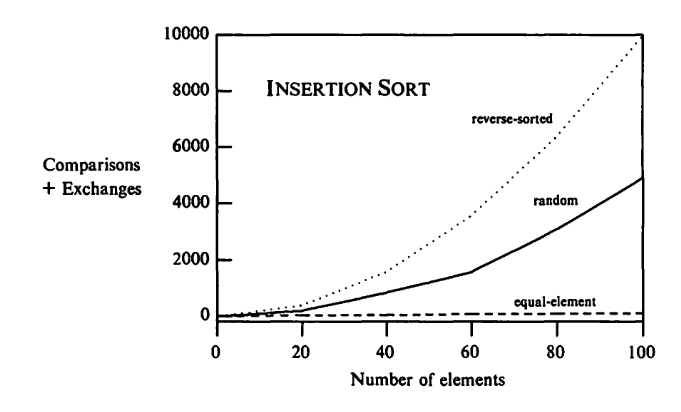
\includegraphics[scale=0.7]{./images/insertion_sort.png}
\end{center}

总得来说, 插入排序适用于元素个数较少的情况, 当元素个数过多时, 该算法
的性能就会快速下降, 除非输入数据基本有序.

通过为每个排序函数添加两个计数器, 我们就可以为上面的图, 以及本章中的
其他图生成所需要的数据. 其中一个计算比较的次数, 另一个计算交换的次数.
这是带计数功能的 \texttt{isort} 函数:
\begin{awkcode}
    function isort(A,n,     i,j,t) {  # insertion sort
        for (i = 2; i <= n; i++)      # with counters
            for (j = i; j > 1 && ++comp &&
              A[j-1] > A[j] && ++exch; j--) {
                # swap A[j-1] and A[j]
                t = A[j-1]; A[j-1] = A[j]; A[j] = t
            }
    }
\end{awkcode}
计数操作都放在内层 \texttt{for} 循环的条件判断部分完成.由 \verb'&&' 
连接的条件判断, 按照从左到右的顺序进行求值, 直到某一项为假. 表达式
\texttt{++comp} 总是为真 (这里必须使用前缀形式的自增运算符), 于是,
数组中的元素每比较一次, \texttt{comp} 的值就加 1, 递增操作在比较之前
完成. 当且仅当某两个元素被交换时, \texttt{exch} 的值才会加 1.
\marginpar{159}

下面的程序用于组织测试, 以及为坐标图准备数据. 同样, 它的功能相当于一
个微型编程语言, 可以灵活地指定参数.
\begin{awkcode}
    # test framework for sort performance evaluation
    #   input:  lines with sort name, type of data, sizes...
    #   output: name, type, size, comparisons, exchanges, c+e

    {   for (i = 3; i <= NF; i++)
            test($1, $2, $i)
    }

    function test(sort, data, n) {
        comp = exch = 0
        if (data ~ /rand/)
            genrand(A, n)
        else if (data ~ /id/)
            genid(A, n)
        else if (data ~ /rev/)
            genrev(A, n)
        else
            print "illegal type of data in", $0
        if (sort ~ /q.*sort/)
            qsort(A, 1, n)
        else if (sort ~ /h.*sort/)
            hsort(A, n)
        else if (sort ~ /i.*sort/)
            isort(A, n)
        else print
            "illegal type of sort in", $0
        print sort, data, n, comp, exch, comp+exch
    }

    # test-generation and sorting routines ...

\end{awkcode}
输入数据是由多行组成的序列, 类似于
\begin{shell}
    isort random 0 20 40 60 80 100 
    isort ident 0 20 40 60 80 100
\end{shell}
输出数据的每一行都包括名字, 类型, 大小, 以及每一种大小的数量.\footnote{
    原文为 And the output consist of lines containing the name, type, size,
and counts for each size.}  输出数据被输送给绘图程序 \texttt{grap}, 它
是我们在第 \ref{chap:little_languages} 章讨论的绘图程序的原始版本.

\begin{exercise}
    实际上, 函数 \texttt{check} 并不是一个很强大的测试, 什么样的错误会
    使它检测失败? 你会如何改进?
\end{exercise}

\begin{exercise}
    我们的大多数测试都基于整数排序, 面对其他类型的数据时, \texttt{isort}
    的表现会如何? 为了处理更一般的数据, 你会如何改进测试框架程序?
\end{exercise}

\begin{exercise}
    我们默认每一种基本操作都需要相同的时间, 也就是说, 访问一个元素, 比较 
    两个元素的值, 加法, 赋值等操作所消耗的时间是相同的. 对于 awk 程序来说 
    这个假设是否合理? 写一个处理大量数据的程序, 来验证你的想法.
\end{exercise}
\marginpar{160}

\subsection{快速排序}
\label{subsec:quicksort}

\cterm{基本概念}. 快速排序是最高效的通用排序算法之一, 由 C. A. R. Hoare
在六十年代早期提出. 为了对一个元素序列进行排序, 快速排序算法把序列划分成
两个子序列, 然后再递归地对子序列进行排序. 在划分阶段, 算法从序列中选取
一个数作为划分点, 把剩下的元素分成两组: 小于划分元素的分在一个组中, 
而大于或等于划分元素的分在另一个组中, 然后再对这两组递归调用快速排序.
如果一个序列所含的元素个数小于2, 则可认为它已经是有序的了, 于是算法
什么也不做就返回.

\cterm{实现}. 实现快速排序有多种方式, 这些方式的不同点就在于划分阶段.
我们所选择的实现方式比较容易理解, 虽然不是最快的. 因为算法是递归的,
所以我们会在划分操作作用在子数组 \texttt{A[left]}, \texttt{A[left+1]},
..., \texttt{A[right]} 上时, 对划分进行描述.

首先需要选择一个划分元素: 从范围 \texttt{[left,right]} 中随机选取一个数
\texttt{r} 作为划分点, 任何一个元素都可以作为划分点, 但是如果序列已经具
有了某种程度上的有序, 那么随机选择的效果会更好. 位置 \texttt{r} 上的元素
\texttt{p} 现在成了划分元素. 交换 \texttt{A[left]} 与 \texttt{A[r]},
在划分的过程中, 数组始终把元素 \texttt{p} 放在 \texttt{A[left]}, 
\texttt{A[left]} 的后面是比 \texttt{p} 小的元素, 再接下来是大于或等于
\texttt{p} 的元素, 最后是到目前为止未处理的元素:
\begin{center}
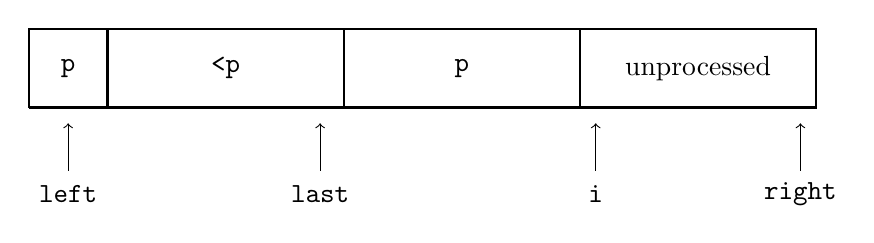
\begin{tikzpicture}
    \draw[thick] (0, 0) -- (0, 1) -- (10, 1) -- (10, 0) -- (0, 0);
    \draw[thick] (1, 0) -- (1, 1);
    \draw[thick] (4, 0) -- (4, 1);
    \draw[thick] (7, 0) -- (7, 1);
    \draw[thick] (7, 0) -- (7, 1);

    \node at (0.5, 0.5) {\texttt{p}};
    \node at (2.5, 0.5) {\texttt{<p}};
    \node at (5.5, 0.5) {\texttt{$\geqslant$p}};
    \node at (8.5, 0.5) {unprocessed};

    \draw[->] (0.5, -0.8) -- (0.5, -0.2);
    \draw[->] (3.7, -0.8) -- (3.7, -0.2);
    \draw[->] (7.2, -0.8) -- (7.2, -0.2);
    \draw[->] (9.8, -0.8) -- (9.8, -0.2);

    \node at (0.5, -1.1) {\texttt{left}};
    \node at (3.7, -1.1) {\texttt{last}};
    \node at (7.2, -1.1) {\texttt{i}};
    \node at (9.8, -1.1) {\texttt{right}};
\end{tikzpicture}
\end{center}

下标 \texttt{last} 指向最后一个比 \texttt{p} 小的元素, 下标 \texttt{i}
指向下一个未处理的元素. 初始化时, \texttt{last} 等于 \texttt{left},
\texttt{i} 等于 \texttt{left+1}.

在划分过程的循环中, 我们比较元素 \texttt{A[i]} 与 \texttt{p}. 如果 
\texttt{A[i]} $\geqslant$ \texttt{p}, 只需要递增 \texttt{i} 即可; 如果
\texttt{A[i]} $<$ \texttt{p},
此时需要递增 \texttt{last}, 并交换 \texttt{A[last]} 与 \texttt{A[i]},
最后再递增 \texttt{i}. 按照这种方式, 一旦所有的元素都处理完毕, 我们需要
交换 \texttt{A[left]} 与 \texttt{A[last]}. 到这里, 我们已经完成了一次
划分, 此时的数组看起来就像这样:
\marginpar{161}
\begin{center}
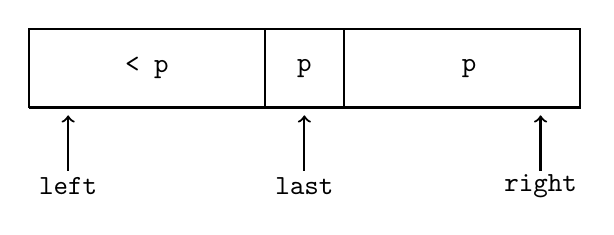
\begin{tikzpicture}
    \draw[thick] (0, 0) -- (0, 1) -- (7, 1) -- (7, 0) -- (0, 0);
    \draw[thick] (3, 0) -- (3, 1);
    \draw[thick] (4, 0) -- (4, 1);

    \draw[thick, ->] (0.5, -0.8) -- (0.5, -0.1);
    \draw[thick, ->] (3.5, -0.8) -- (3.5, -0.1);
    \draw[thick, ->] (6.5, -0.8) -- (6.5, -0.1);

    \node at (0.5, -1.0) {\texttt{left}};
    \node at (3.5, -1.0) {\texttt{last}};
    \node at (6.5, -1.0) {\texttt{right}};
    \node at (1.5, 0.5) {\texttt{< p}};
    \node at (3.5, 0.5) {\texttt{p}};
    \node at (5.5, 0.5) {\texttt{$\geqslant$ p}};
\end{tikzpicture}
\end{center}
现在, 我们对左边的子数组与右边的子组执行同样的操作.

假设我们对下列8个元素进行快速排序:
\begin{file}
    8 1 6 3 5 2 4 7
\end{file}
第一步我们可能选择 4 作为划分元素, 接下来, 划分操作会把数组重新排列成
\begin{file}
    2 1 3|4|5 6 8 7
\end{file}
然后再递归地对子数组 \texttt{2 1 3} 与 \texttt{5 6 8 7} 进行快速排序,
当子数组的元素个数少于 2 时, 递归过程就会停止.

下面程序所包含的函数 \texttt{qsort} 实现了快速排序算法, 我们可以用插入排序
的测试例程对该程序进行测试.
\begin{awkcode}
    # quicksort

        { A[NR] = $0 }

    END { qsort(A, 1, NR)
          for (i = 1; i <= NR; i++)
              print A[i]
        }

    # qsort - sort A[left..right] by quicksort

    function qsort(A,left,right,   i,last) {
         if (left >= right)  # do nothing if array contains
             return          # less than two elements
         swap(A, left, left + int((right-left+1)*rand()))
         last = left   # A[left] is now partition element
         for (i = left+1; i <= right; i++)
             if (A[i] < A[left])
                 swap(A, ++last, i)
         swap(A, left, last)
         qsort(A, left, last-1)
         qsort(A, last+1, right)
    }

    function swap(A,i,j,   t) {
         t = A[i]; A[i] = A[j]; A[j] = t
    }
\end{awkcode}

\cterm{性能}. \texttt{qsort} 所执行的操作次数取决于数组划分时的均匀程度.
如果数组划分每次都很平均, 那么程序的运行时间与 $n \log n$ 成正比.
\marginpar{162}
于是, 如果数据规模变为原来的两倍, 那么程序的运行时间只会在原来两倍的基础上
再稍微多出一点.

在最坏的情况下, 划分操作的结果会出现其中一个子数组长度为 0 的情况, 比如,
当所有元素都相同时, 就会出现这种情况. 这时候, 快速排序的时间复杂度就
会退化到二次方. 幸运的是, 对于随机数据来说, 不会出现这种极不均匀的划分. 
下面这张图显示了快速排序面对三种类型的输入数据时的性能表现 (在测试插入
排序时, 也用到了这三种类型的数据). 正如你所看到的那样, 对于同元素序列
来说, 操作次数的增长速度要比另外两种类型的增长速度快得多. \footnote{应该 
用矢量图, 而不是从原版中截图 --- 译者注}

\begin{center}
    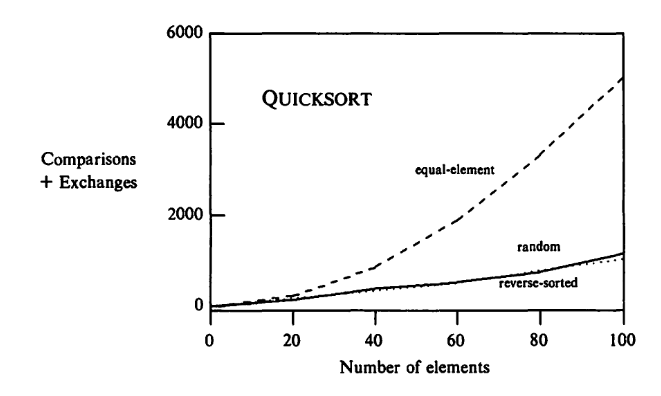
\includegraphics[scale=0.7]{images/quicksort.png}
\end{center}

\begin{exercise}
    为 \texttt{qsort} 添加计数语句, 计算比较操作和交换操作的执行次数.
    你得到的结果是否和我们的类似 ?
\end{exercise}

\begin{exercise}
    记录程序的运行时间, 而不是操作次数. 运行时间的统计图是否和操作次数
    的相同 ? 用大一点的例子作测试, 看看其统计图还是不是一样的.
\end{exercise}

\subsection{堆排序}
\label{subsec:heapsort}

\cterm{基本概念}. \cterm{优先级队列} (\term{priority queue}) 是一种数据
结构, 用于存储和检索元素. 它有两种基本操作: 往队列中插入一个新元素, 以及 
从队列中提取最大的元素. 这表明优先级队列可以用来排序: 首先把所有的元素
插入到队列中, 然后每次抽取一个元素. 因为每次移除的都是最大的元素, 所以 
元素是以降序地方式从队列中抽取出来. 这种排序方法叫作堆排序, 由
J. W. J. Williams 和 R. W. Floyd 在 60 年代早期提出.

\marginpar{163}
堆排序使用一种称为 \cterm{堆} (\term{heap}) 的数据结构来维护优先级队列,
我们可以把堆想像成一棵二叉树, 但是带有两条额外的性质:
\begin{enumerate}
    \item 树是高度平衡的: 叶子结点最多只在两个不同的层次上出现, 另外,
        位于最底层 (距离根结点最远的层次) 的叶子尽量靠左排列;
    \item 树是部分有序的: 每个结点的值大于或等于它的孩子结点.
\end{enumerate}
这是带有 10 个元素的堆:\footnote{TODO}

堆具有两条非常重要的性质. 第一条性质是, 如果有 \textit{n} 个结点, 那么所
有的从根结点到叶子结点的路径长度都不会大于 $\log_2 n$. 第二条性质是,
具有最大值的元素总是在根结点 (这个位置称为 ``堆顶'').

如果我们用一个数组 \texttt{A} 来模拟堆, 那么就不需要构造显式的二叉树.
树中的结点按照宽度优先遍历的顺序出现在数组中, 也就是说, 根结点在 
\texttt{A[1]}, 它的左孩子与右孩子分别在 \texttt{A[2]} 和 \texttt{A[3]}.
总的来说, 如果某个结点在 \texttt{A[}\textit{i}\texttt{]}, 那么它的孩子就
在 \texttt{A[2}\textit{i}\texttt{]} 和 \texttt{A[2}\textit{i}\texttt{+1]},
如果只有一个孩子的话, 那就在 \texttt{A[2}\textit{i}\texttt{]}.
于是, 上面那棵树对应的数组 \texttt{A} 就是:\footnote{TODO}

堆的部分有序性质指的是元素 \texttt{A[}\textit{i}\texttt{]} 大于或等于
它的孩子结点 \texttt{A[2}\textit{i}\texttt{]} 与
\texttt{A[2}\textit{i}\texttt{+1]}, 如果只有一个孩子的话, 就那大于或等于
\texttt{A[2}\textit{i}\texttt{]}. 如果某个数组满足这个条件, 我们就说
这个数组具有 ``堆属性''.

\cterm{实现} (\term{Implementation}). 堆排序由两个阶段组成: 构造堆, 以及 
按顺序从堆中提取元素. 两个阶段都要调用函数 \texttt{heapify(A,i,j)}, 使得
子数组 \texttt{A[i]}, \texttt{A[i+1]}, ..., \texttt{A[j]} 具有堆属性 (假设 
\texttt{A[i+1]}, ..., \texttt{A[j]} 已经具有了堆属性). \texttt{heapify}
的基本操作是比较 \texttt{A[i]} 与它的孩子, 如果 \texttt{A[i]} 没有孩子,
或者比它的孩子大, 那么函数就直接返回; 否则, 交换 \texttt{A[i]} 和它的最
大孩子, 然后再对孩子重复这个基本操作.

在第一个阶段, 堆排序通过调用
\texttt{heapify(A,}\textit{i}\texttt{,}\textit{n}\texttt{)} (\textit{i} 从
\textit{n}/2 递减到 1), 把数组转化成一个堆.

\marginpar{164}
第2个阶段开始时, \textit{i} 被赋值为 \textit{n}, 然后重复执行以下三个
步骤: 首先, 把堆的最大元素 \texttt{A[1]} 与 \texttt{A[}\textit{i}\texttt{]}
作交换, \texttt{A[}\textit{i}\texttt{]} 是堆中最靠右的元素. 然后, 堆的 
元素个数减 1 (即 \textit{i} 减 1). 这两个步骤相当于从堆中移除最大元素.
注意到, 这样做的结果是数组中最后的
\textit{n}\texttt{-}\textit{i}\texttt{+1} 个元素处于有序状态. 最后,
对数组 \texttt{A} 的前 \textit{i}\texttt{-1} 个元素调用
\texttt{heapify(A,1,}\textit{i}\texttt{-1)}.

这三个步骤一直重复到堆中只剩下一个元素为止, 而这个元素其实就是序列中的
最小值. 由于数组中剩下的元素按照升序排列, 所以当操作结束时, 序列就是有
序的了. 在操作过程中, 数组看起来就像这样:
\begin{center}
    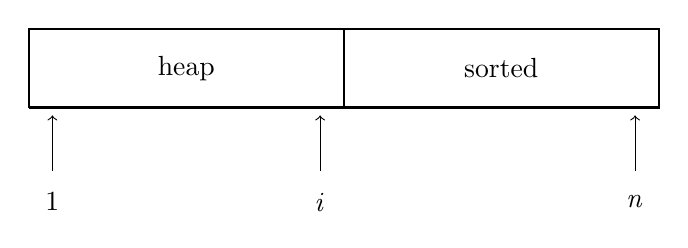
\begin{tikzpicture}
        \draw[thick] (0, 0) -- (0, 1) -- (8, 1) -- (8, 0) -- (0, 0);
	\draw[thick] (4, 0) -- (4, 1);
	\draw[->] (0.3, -0.8) -- (0.3, -0.1);
	\draw[->] (3.7, -0.8) -- (3.7, -0.1);
	\draw[->] (7.7, -0.8) -- (7.7, -0.1);
	\node at (2, 0.5) {heap};
	\node at (6, 0.5) {sorted};
	\node at (0.3, -1.2) {1};
	\node at (3.7, -1.2) {\textit{i}};
	\node at (7.7, -1.2) {\textit{n}};
    \end{tikzpicture}
\end{center}
数组中从 1 到 \textit{i} 的元素具有堆属性, 从 \textit{i}\texttt{+1} 到 
\textit{n} 是数组中最大的 \textit{n}\texttt{-}\textit{i} 个元素,
按照升序排列.
开始时, \textit{i}=\textit{n}, 因此数组中没有已排好序的部分.

考虑上面展示的元素所组成的数组, 该数组已经具有堆属性. 在第二个阶段的第
一个步骤, 我们交换元素 \texttt{76} 和 \texttt{28}:
\begin{file}
    28 72 34 59 63 17 29 37 33 | 76
\end{file}
在第 2 个步骤, 我们把堆的大小递减到 9. 然后在第 3 个步骤中, 通过一系列的
交换操作, 把 \texttt{28} 移动到合适的位置, 从而维持住前 9 个元素的堆属性:
\begin{file}
    72 63 34 59 28 17 29 37 33 | 76
\end{file}
我们可以把这个过程可视化: 让元素 \texttt{28} 沿着二叉树的路径, 从根结点
开始, 朝着叶子结点方向, 逐渐向下渗透, 直到到达一个这样的结点: 它的孩子 
小于或等于 \texttt{28}:\footnote{TODO}

在下一次迭代中, 第一个步骤交换元素 \texttt{72} 和 \texttt{33}:
\begin{file}
    33 63 34 59 28 17 29 37 | 72 76
\end{file}
第二个步骤把 \textit{i} 递减到 8, 第三次迭代把 \texttt{33} 移动到合适的 
位置:
\marginpar{165}
\begin{file}
    63 59 34 37 28 17 29 33 | 72 76
\end{file}
下一次迭代以交换 \verb'63' 与 \verb'33' 作为开始, 迭代结束时, 序列变成:
\begin{file}
    59 37 34 33 28 17 29 | 63 72 76
\end{file}
当数组处于有序状态时, 迭代过程结束.

下面的程序对输入数据按照升序进行排列, 使用的正是上面提到的过程. 我们把 
大部分的, 由单独一条表达式组成的语句用花括号包围起来, 至于这样做的原因
将会在下一节讨论刻画时说明.
\begin{awkcode}
    # heapsort

        { A[NR] = $0 }

    END { hsort(A, NR)
          for (i = 1; i <= NR; i++)
              { print A[i] }
        }

    function hsort(A,n,  i) {
        for (i = int(n/2); i >= 1; i--)  # phase 1
             { heapify(A, i, n) }
        for (i = n; i > 1; i--) {        # phase 2
             { swap(A, 1, i) }
             { heapify(A, 1, i-1) }
        }
    }
    function heapify(A,left,right,   p,c) {
        for (p = left; (c = 2*p) <= right; p = c) {
            if (c < right && A[c+1] > A[c])
                { c++ }
            if (A[p] < A[c])
                { swap(A, c, p) }
        }
    }
    function swap(A,i,j,   t) {
        t = A[i]; A[i] = A[j]; A[j] = t
    }
\end{awkcode}

\cterm{性能}. \verb'hsort' 总的操作次数正比于 $n\log n$, 即使是在最坏的
情况下也是如此. 同样, 我们用三种类型的元素序列对 \verb'hsort' 进行性能
测试, 下面这张图显示了测试结果, 可以看到, \verb'hsort' 面对相同元素序列
时, 性能优于快速排序.\footnote{应该用矢量图}
\marginpar{166}
\begin{center}
    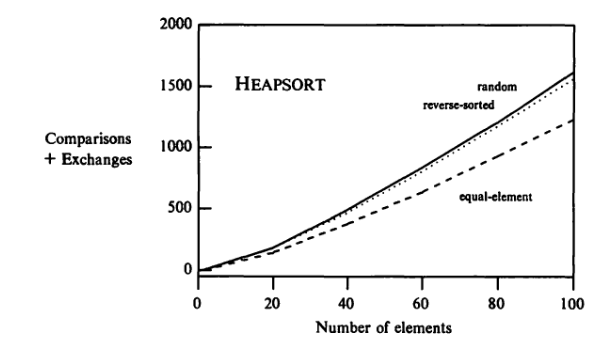
\includegraphics[scale=0.7]{images/heap_sort.png}
\end{center}

接下来的这张图显示了本节所讨论的三种排序算法, 在面对随机输入数据时的性能
表现.
\begin{center}
    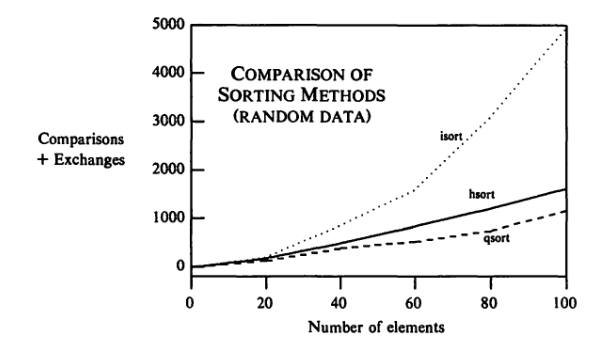
\includegraphics[scale=0.7]{images/sort_cmp.png}
\end{center}

前面曾经说过, \texttt{isort} 对随机数据进行排序的时间复杂度是二次的, 而
\texttt{hsort} 与 \texttt{qsort} 的复杂度却是 $n \log n$. 这张图清楚地
展示了一个优秀算法的重要性: 随着数据规模的增加, 二次方程序的性能与
$n \log n$ 程序性能之间的差距急剧加大.
\marginpar{167}
\begin{exercise}
    \texttt{check} 总是发现 \texttt{isort} 的输出是有序的. 对于
    \texttt{qsort} 与 \texttt{hsort} 是否也成立 ? 如果输入数据仅仅由
    数值组成, 或者是一些看起来不太像数值的字符串, 那么是否还成立 ?
\end{exercise}
